\begin{figure}[H]
    \centering
    \tikzset{every picture/.style={line width=0.75pt}} %set default line width to 0.75pt        
    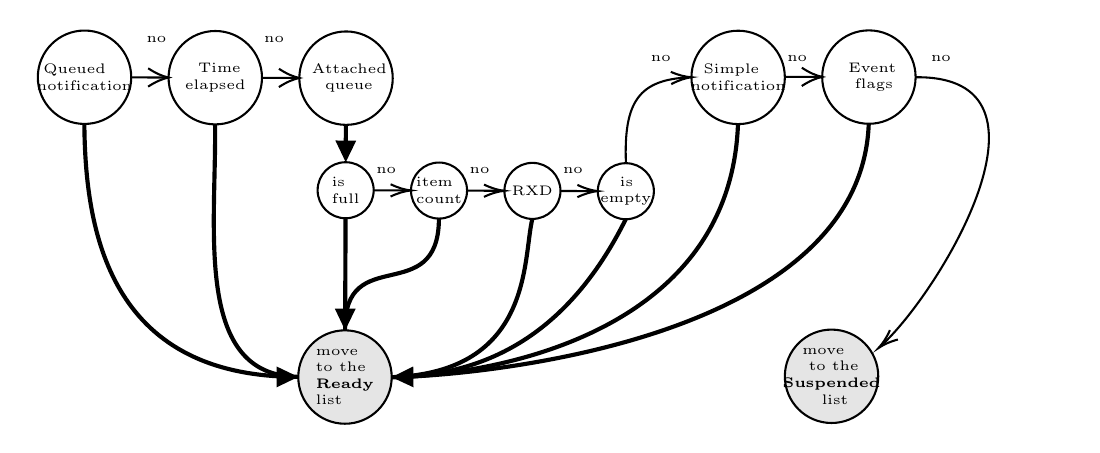
\begin{tikzpicture}[x=0.75pt,y=0.75pt,yscale=-0.9,xscale=0.9]
        \draw   (85.09,90) .. controls (71.28,89.95) and (60.05,101.11) .. (60,114.91) .. controls (59.95,128.72) and (71.11,139.95) .. (84.91,140) .. controls (98.72,140.05) and (109.95,128.89) .. (110,115.09) .. controls (110.05,101.28) and (98.89,90.05) .. (85.09,90) -- cycle ;
        \draw   (155.09,90.24) .. controls (141.28,90.2) and (130.05,101.35) .. (130,115.16) .. controls (129.95,128.96) and (141.11,140.2) .. (154.91,140.24) .. controls (168.72,140.29) and (179.95,129.14) .. (180,115.33) .. controls (180.05,101.52) and (168.89,90.29) .. (155.09,90.24) -- cycle ;
        \draw    (110,115.09) -- (128,115.15) ;
        \draw [shift={(130,115.16)}, rotate = 180.2] [color={rgb, 255:red, 0; green, 0; blue, 0 }  ][line width=0.75]    (10.93,-4.9) .. controls (6.95,-2.3) and (3.31,-0.67) .. (0,0) .. controls (3.31,0.67) and (6.95,2.3) .. (10.93,4.9)   ;
        \draw   (224.84,160.49) .. controls (216.56,160.46) and (209.82,167.15) .. (209.79,175.44) .. controls (209.76,183.72) and (216.45,190.46) .. (224.74,190.49) .. controls (233.02,190.52) and (239.76,183.82) .. (239.79,175.54) .. controls (239.82,167.26) and (233.13,160.52) .. (224.84,160.49) -- cycle ;
        \draw [line width=1.5]    (84.91,140) .. controls (85.37,197.92) and (98.51,274.01) .. (196.45,275.38) ;
        \draw [shift={(199.44,275.4)}, rotate = 539.9200000000001] [fill={rgb, 255:red, 0; green, 0; blue, 0 }  ][line width=0.08]  [draw opacity=0] (11.61,-5.58) -- (0,0) -- (11.61,5.58) -- cycle    ;
        \draw   (225.09,90.49) .. controls (211.28,90.44) and (200.05,101.59) .. (200,115.4) .. controls (199.95,129.21) and (211.1,140.44) .. (224.91,140.49) .. controls (238.72,140.54) and (249.95,129.38) .. (250,115.58) .. controls (250.05,101.77) and (238.89,90.54) .. (225.09,90.49) -- cycle ;
        \draw    (180,115.33) -- (198,115.39) ;
        \draw [shift={(200,115.4)}, rotate = 180.2] [color={rgb, 255:red, 0; green, 0; blue, 0 }  ][line width=0.75]    (10.93,-4.9) .. controls (6.95,-2.3) and (3.31,-0.67) .. (0,0) .. controls (3.31,0.67) and (6.95,2.3) .. (10.93,4.9)   ;
        \draw [line width=1.5]    (224.91,140.49) -- (224.86,156.49) ;
        \draw [shift={(224.84,160.49)}, rotate = 270.2] [fill={rgb, 255:red, 0; green, 0; blue, 0 }  ][line width=0.08]  [draw opacity=0] (11.61,-5.58) -- (0,0) -- (11.61,5.58) -- cycle    ;
        \draw   (274.84,160.66) .. controls (266.56,160.63) and (259.82,167.33) .. (259.79,175.61) .. controls (259.76,183.89) and (266.45,190.63) .. (274.74,190.66) .. controls (283.02,190.69) and (289.76,184) .. (289.79,175.72) .. controls (289.82,167.43) and (283.13,160.69) .. (274.84,160.66) -- cycle ;
        \draw    (239.79,175.54) -- (257.79,175.6) ;
        \draw [shift={(259.79,175.61)}, rotate = 180.2] [color={rgb, 255:red, 0; green, 0; blue, 0 }  ][line width=0.75]    (10.93,-3.29) .. controls (6.95,-1.4) and (3.31,-0.3) .. (0,0) .. controls (3.31,0.3) and (6.95,1.4) .. (10.93,3.29)   ;
        \draw   (324.84,160.84) .. controls (316.56,160.81) and (309.82,167.5) .. (309.79,175.79) .. controls (309.76,184.07) and (316.45,190.81) .. (324.74,190.84) .. controls (333.02,190.87) and (339.76,184.17) .. (339.79,175.89) .. controls (339.82,167.61) and (333.13,160.87) .. (324.84,160.84) -- cycle ;
        \draw [line width=1.5]    (224.74,190.49) -- (224.54,246.49) ;
        \draw [shift={(224.53,250.49)}, rotate = 270.2] [fill={rgb, 255:red, 0; green, 0; blue, 0 }  ][line width=0.08]  [draw opacity=0] (11.61,-5.58) -- (0,0) -- (11.61,5.58) -- cycle    ;
        \draw  [fill=gray!20  ,fill opacity=1 ] (224.53,250.49) .. controls (210.72,250.44) and (199.49,261.59) .. (199.44,275.4) .. controls (199.39,289.21) and (210.55,300.44) .. (224.35,300.49) .. controls (238.16,300.54) and (249.39,289.38) .. (249.44,275.57) .. controls (249.49,261.77) and (238.33,250.54) .. (224.53,250.49) -- cycle ;
        \draw   (435,90.09) .. controls (421.19,90.04) and (409.96,101.19) .. (409.91,115) .. controls (409.86,128.81) and (421.02,140.04) .. (434.83,140.09) .. controls (448.63,140.14) and (459.86,128.98) .. (459.91,115.17) .. controls (459.96,101.37) and (448.81,90.14) .. (435,90.09) -- cycle ;
        \draw    (289.79,175.72) -- (297.46,175.74) -- (307.79,175.78) ;
        \draw [shift={(309.79,175.79)}, rotate = 180.2] [color={rgb, 255:red, 0; green, 0; blue, 0 }  ][line width=0.75]    (10.93,-3.29) .. controls (6.95,-1.4) and (3.31,-0.3) .. (0,0) .. controls (3.31,0.3) and (6.95,1.4) .. (10.93,3.29)   ;
        \draw [line width=1.5]    (154.91,140.24) .. controls (155.5,197) and (143.5,275) .. (199.44,275.4) ;
        \draw [line width=1.5]    (274.74,190.66) .. controls (274.5,239) and (223.5,203) .. (224.53,250.49) ;
        \draw [line width=1.5]    (324.74,190.84) .. controls (319.5,212) and (325.5,273) .. (249.44,275.57) ;
        \draw   (374.84,161.01) .. controls (366.56,160.98) and (359.82,167.68) .. (359.79,175.96) .. controls (359.76,184.24) and (366.45,190.98) .. (374.74,191.01) .. controls (383.02,191.04) and (389.76,184.35) .. (389.79,176.06) .. controls (389.82,167.78) and (383.13,161.04) .. (374.84,161.01) -- cycle ;
        \draw    (339.79,175.89) -- (357.79,175.95) ;
        \draw [shift={(359.79,175.96)}, rotate = 180.2] [color={rgb, 255:red, 0; green, 0; blue, 0 }  ][line width=0.75]    (10.93,-3.29) .. controls (6.95,-1.4) and (3.31,-0.3) .. (0,0) .. controls (3.31,0.3) and (6.95,1.4) .. (10.93,3.29)   ;
        \draw [line width=1.5]    (374.74,191.01) .. controls (342.17,256.37) and (296.35,273.96) .. (253.42,275.48) ;
        \draw [shift={(249.44,275.57)}, rotate = 359.25] [fill={rgb, 255:red, 0; green, 0; blue, 0 }  ][line width=0.08]  [draw opacity=0] (11.61,-5.58) -- (0,0) -- (11.61,5.58) -- cycle    ;
        \draw    (374.84,161.01) .. controls (373.53,127.68) and (382.14,116.45) .. (408.29,115.07) ;
        \draw [shift={(409.91,115)}, rotate = 537.9100000000001] [color={rgb, 255:red, 0; green, 0; blue, 0 }  ][line width=0.75]    (10.93,-3.29) .. controls (6.95,-1.4) and (3.31,-0.3) .. (0,0) .. controls (3.31,0.3) and (6.95,1.4) .. (10.93,3.29)   ;
        \draw   (505,89.91) .. controls (491.19,89.86) and (479.96,101.02) .. (479.91,114.83) .. controls (479.86,128.63) and (491.02,139.86) .. (504.83,139.91) .. controls (518.63,139.96) and (529.86,128.81) .. (529.91,115) .. controls (529.96,101.19) and (518.81,89.96) .. (505,89.91) -- cycle ;
        \draw    (459.91,114.76) -- (477.91,114.82) ;
        \draw [shift={(479.91,114.83)}, rotate = 180.2] [color={rgb, 255:red, 0; green, 0; blue, 0 }  ][line width=0.75]    (10.93,-4.9) .. controls (6.95,-2.3) and (3.31,-0.67) .. (0,0) .. controls (3.31,0.67) and (6.95,2.3) .. (10.93,4.9)   ;
        \draw [line width=1.5]    (434.83,140.09) .. controls (430.5,257) and (293.5,275) .. (249.44,275.57) ;
        \draw [line width=1.5]    (504.83,139.91) .. controls (500.5,256.83) and (293.5,275) .. (249.44,275.57) ;
        \draw  [fill=gray!20 ] (485,250.09) .. controls (471.19,250.04) and (459.96,261.19) .. (459.91,275) .. controls (459.86,288.81) and (471.02,300.04) .. (484.83,300.09) .. controls (498.63,300.14) and (509.86,288.98) .. (509.91,275.17) .. controls (509.96,261.37) and (498.81,250.14) .. (485,250.09) -- cycle ;
        \draw    (529.91,115) .. controls (613.23,114.01) and (542.77,230.26) .. (511.41,258.76) ;
        \draw [shift={(510,260)}, rotate = 319.45] [color={rgb, 255:red, 0; green, 0; blue, 0 }  ][line width=0.75]    (10.93,-3.29) .. controls (6.95,-1.4) and (3.31,-0.3) .. (0,0) .. controls (3.31,0.3) and (6.95,1.4) .. (10.93,3.29)   ;
        \draw (85,115) node  [font=\tiny] [align=left] { \ Queued\\notification};
        \draw (224.79,175.49) node  [font=\tiny] [align=left] {is\\full};
        \draw (274.79,175.66) node  [font=\tiny] [align=left] {item\\count};
        \draw (324.79,175.84) node  [font=\tiny] [align=left] {RXD};
        \draw (224.44,275.49) node  [font=\tiny] [align=left] {move \\to the\\\textbf{Ready} \\list};
        \draw (374.79,176.01) node  [font=\tiny] [align=left] { \ \ \ is\\empty};
        \draw (155,115.24) node  [font=\tiny] [align=left] { \ \ Time\\elapsed};
        \draw (225,115.49) node  [font=\tiny] [align=left] { \ Attached\\ \ \ \ queue};
        \draw (434.91,115.09) node  [font=\tiny] [align=left] { \ \ Simple\\notification};
        \draw (504.91,114.91) node  [font=\tiny] [align=left] { \ Event\\ \ \ flags};
        \draw (484.91,275.09) node  [font=\tiny] [align=left] { \ \ \ move \\ \ \ \ \ to the\\\textbf{Suspended} \\ \ \ \ \ \ \ list};
        \draw (123.5,95) node  [font=\tiny] [align=left] {no};
        \draw (186.5,95) node  [font=\tiny] [align=left] {no};
        \draw (246.5,165) node  [font=\tiny] [align=left] {no};
        \draw (296.5,165) node  [font=\tiny] [align=left] {no};
        \draw (346.5,165) node  [font=\tiny] [align=left] {no};
        \draw (393.5,105) node  [font=\tiny] [align=left] {no};
        \draw (466.5,105) node  [font=\tiny] [align=left] {no};
        \draw (543.5,105) node  [font=\tiny] [align=left] {no};
    \end{tikzpicture}
    \caption{Event precedence}
    \label{fig:eventprecedence}
\end{figure}